\documentclass{scrreprt}
\usepackage{graphicx}
\usepackage{amssymb}
\usepackage[encapsulated]{CJK}
\usepackage{listings}
\usepackage{underscore}
\usepackage[bookmarks=true]{hyperref}
\usepackage[utf8]{inputenc}
\usepackage[english]{babel}
\hypersetup{
    bookmarks=false,    % show bookmarks bar?
    pdftitle={Software Requirement Specification},    % title
    pdfauthor={Jean-Philippe Eisenbarth},                     % author
    pdfsubject={TeX and LaTeX},                        % subject of the document
    pdfkeywords={TeX, LaTeX, graphics, images}, % list of keywords
    colorlinks=true,       % false: boxed links; true: colored links
    linkcolor=blue,       % color of internal links
    citecolor=black,       % color of links to bibliography
    filecolor=black,        % color of file links
    urlcolor=purple,        % color of external links
    linktoc=page            % only page is linked
}%
\def\myversion{1.0 }
\date{}
%\title
\usepackage{hyperref}
\begin{document}
\begin{CJK*}{UTF8}{bsmi}
\begin{flushright}
    \rule{16cm}{5pt}\vskip1cm
    \begin{bfseries}
        \Huge{SOFTWARE REQUIREMENTS \\SPECIFICATION}\\
        \vspace{1.9cm}
        for\\
        \vspace{1.9cm}
        貓狗辨識系統\\
        \vspace{1.9cm}
        \Large {Prepared by 1051433 葛東昇 1051514 沈家葳\\1053344 高浩然 1053348 黃世旻}\\
        \vspace{3.8cm}
        開放平台第9組\\
        \vspace{1.9cm}
        June 21, 2019\\
    \end{bfseries}
\end{flushright}

\tableofcontents



\chapter{Introduction}

\section{Purpose}
  這個貓狗辨識系統主要是參考老師之前講解期末所提到的一個範例,並希望能用上課所提到的內容實做出一個可以辨識貓跟狗的程式。


\section{Intended Audience and Reading Suggestions }
  整個SRS文件分成幾個部分,內容包含IntroductionOverall Description、External Interface Requirements、System Features、Other Nonfunctional Requirements等五大部分。Introduction主 要是針對這個系統做出介紹;Overall Description 對程式本身進行介紹;External Interface Requirements 會對Interface進行介紹;System Features 對整個系統功能需求進行講解;Other Nonfunctional Requirements 敘述一些系統額外的需求。
\section{Project Scope}
  現今的社會中,多數人都會經常對著手機跟電腦,逛社群軟體、網拍、玩遊戲等等,變得不常接觸有生命的東西,每天都對著螢幕來了解社會正在發生的問題,但沒有發現一個重要的事情,就是平常生活在我們身邊的毛孩子是狗還是貓。\\
	\\
  所以我們撰寫了一個可以分貓跟狗的程式,方便那些不太能辨認動物的飼主來了解自己身邊的毛小孩,只要上傳自己身邊動物的照片,系統便可以幫助飼主判斷所養的是狗或是貓。\\
	\\
  這個系統在未來我相信會佔到很重要的位子,假使寵物狗走失,巷口的監視器便可以幫忙過濾動物的樣子,不用去用人眼判斷經過的是貓或是狗,得到狗的樣子再來進一步搜尋,可以大大減少找走失的寵物的時間。\\



\chapter{Overall Description}

\section{Product Perspective}
  整體而言,本系統的主要目標是,提出一套貓狗辨識系統,使用卷積神經網路(Convolutional Neural Network,CNN)進行分析,會回傳兩個浮點數,第0個是貓,第1個是狗,貓的數值越大比狗大就是比較偏向貓,反之亦然。
本系統按Fig.\,\ref{fig:2.1} 所示,分成三個部份實行,分別為貓狗資料庫、貓狗分辨模型輸出結果,逐步完成。三個部分的實現內容,概略說明如下:\\
\begin{figure}[h]
\begin{center}
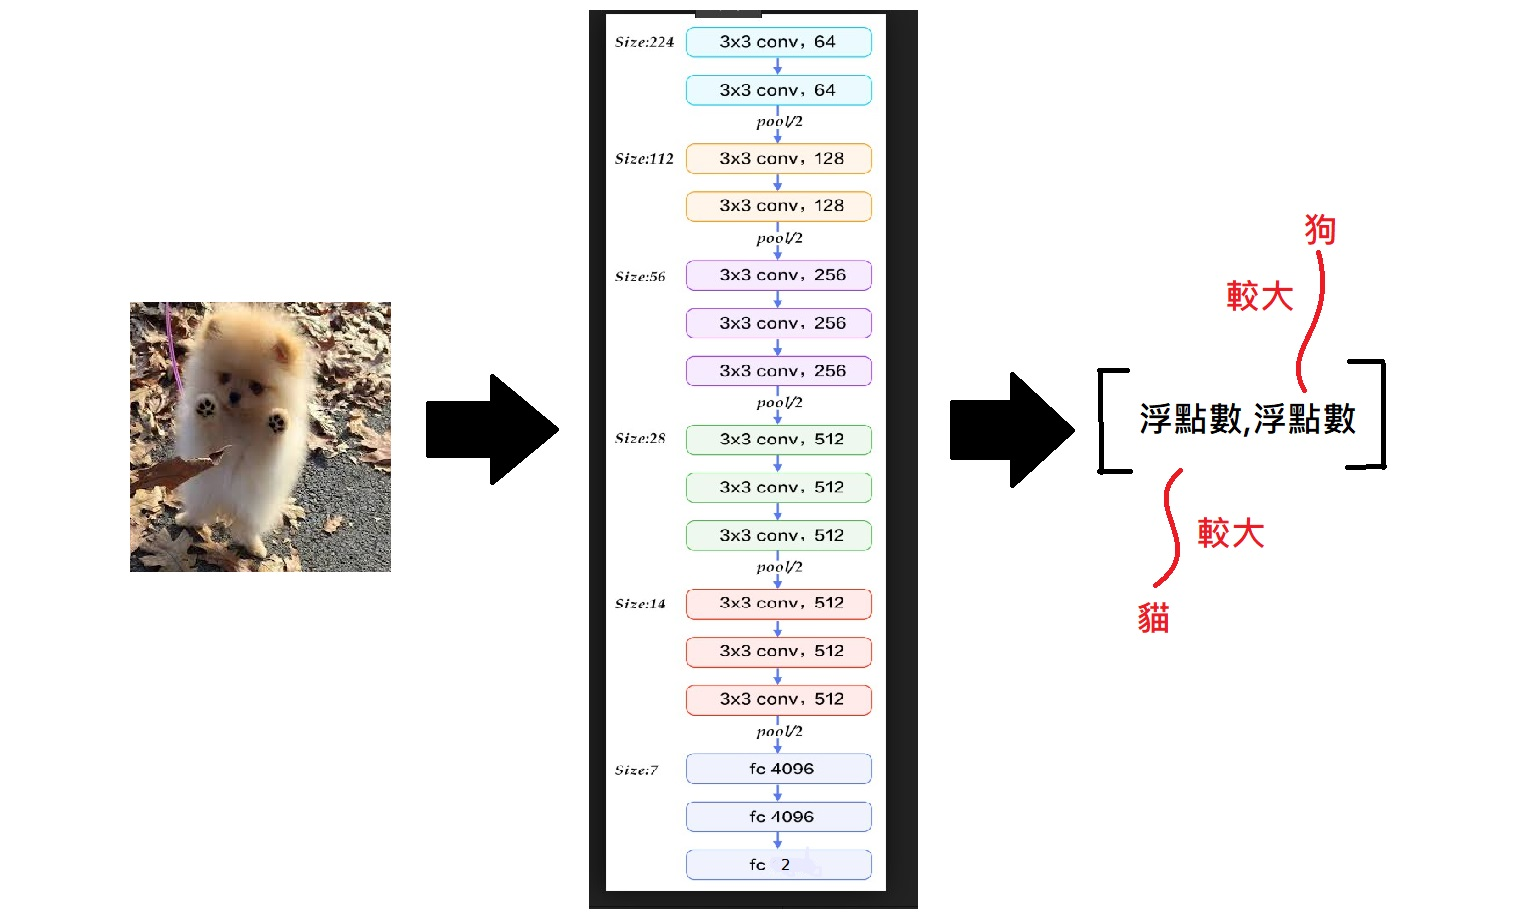
\includegraphics[width=12cm]{Fig.jpg} 
\end{center} 
\label{fig:2.1} 
\caption{簡易流程圖.} 
\end{figure}

\section{Product Functions}
  適用於各式品種的貓狗: 在資料庫的部分,我們蒐集各種品種、顏色的貓狗,並且在pycharm上執行的時候,先輸入我們測試的圖片,並判斷出圖片中的動物是貓還是狗。

\section{User Classes and Characteristics}


\section{Operating Environment}


\section{Operating Environment}


\section{Assumptions and Dependencies}




\chapter{External Interface Requirements}

\section{User Interfaces}


\section{Hardware Interfaces}


\section{Software Interfaces}
\begin{enumerate}
	\item 安裝軟體:\\pytorch、matplotlib、numpy
	\item 使用的參數:\\loss
	\item 輸入與輸出的圖片:
	\begin{enumerate}
		\item 輸入圖片:  貓狗圖像
		\item 輸出圖片 : 
	\end{enumerate}
	\item 輸入與輸出的圖片:
	\begin{enumerate}
		\item 輸入圖片大小 :  224*224
		\item 輸出圖片大小 :  224*224 
	\end{enumerate}
\end{enumerate}



\chapter{System Features}

\section{Description and Priority}


\section{Stimulus/Response Sequences}


\section{Functional Requirements}




\chapter{Other Nonfunctional Requirements}

\section{Performance Requirements}


\section{Safety Requirements} 

\section{Security Requirements}


\end{CJK*}
\end{document}
